\documentclass[12pt]{article}
\usepackage[utf8]{inputenc}
\usepackage{graphics}
\usepackage{graphicx}
\usepackage{float}
\usepackage{eso-pic}
\usepackage[top=3cm,bottom=3cm,left=2.5cm,right=2.5cm,headsep=10pt,letterpaper]{geometry}
\usepackage{verbatim}
\usepackage{amssymb}
\usepackage{stmaryrd}
\usepackage{mathrsfs, amsmath}
\usepackage{listings}
\usepackage{indentfirst}
\usepackage{tabularx}
\usepackage{hyperref}
\lstset{language = MATLAB}
\usepackage{abstract}
\usepackage{amsmath}
\usepackage{amsthm}
\usepackage{tcolorbox}
\usepackage{enumitem}

\begin{document}

\newpage
\newpage
\newtheorem{theorem}{Theorem}

\begin{titlepage}

    \begin{center}
        \vspace*{2.5in}
            \huge
            \textbf{{Homework 3}}\\
            \large
            \textbf{Numerical PDEs}\\
    \end{center}
    ~\vfill
    \noindent \textsc{Colorado School of Mines}\\
    \textsc{Department of Applied Mathematics and Statistics}\\
    
    \vspace{1cm}
    \noindent \textsc{\textbf{AUTHOR INFORMATION}}\\
    \noindent Hugh Scribner\footnote{Computational and Applied Mathematics}\\ 
    \vspace{1mm}
    
\end{titlepage}

\newpage

\tableofcontents

\newpage

\newpage
\section{Problem 1}
 \begin{tcolorbox}
        \textbf{Problem Statement:}\\
        Solve the heat equation using finite differences on a 64x64 and 128x128 grid using Forward Euler, Backward Euler, Runge-Kutta 2, Backward Difference Formula 2, Crank-Nicolson, and RK4. Make convergence plots for each of the methods to see how they perform.
    \end{tcolorbox}
    
    \textbf{Solution:}\\
    To confirm that each of the methods we implemented are converging as expected, each method was used to solve a heat equation on a 64x64 and 128x128 grid, $t \in [0,2\pi]$ for a variety of step sizes. Relative error in the exact solution is shown below. Note that implicit methods (BE, CN, and BDF2) each provided a convergent solution to the PDE regardless of step size, while explicit methods (FE, and RK2) did not provide convergent solutions until a test was run such that the time step satisfied the CFL condition.
        \begin{figure}[H]
        \begin{centering}
            \centering
                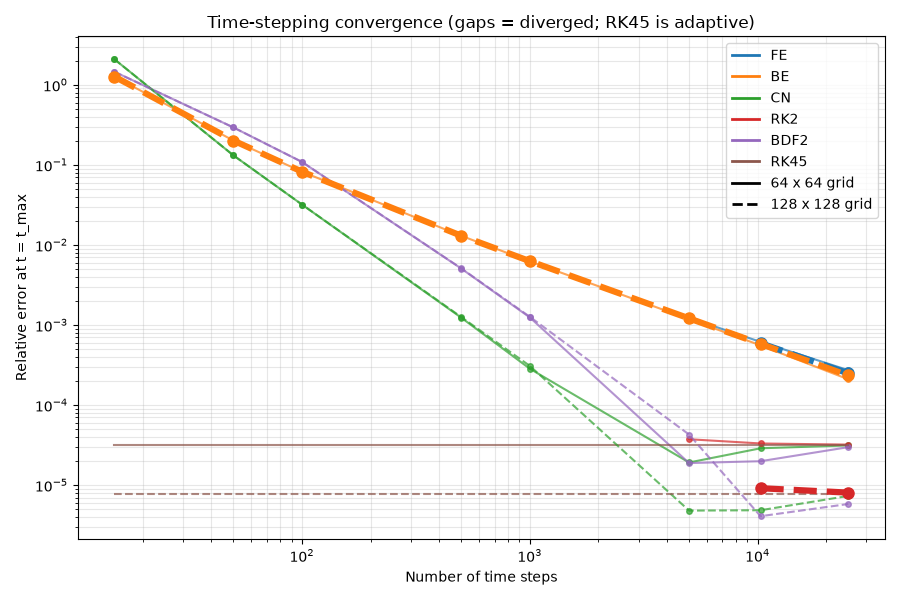
\includegraphics[scale=.7]{Images/convergence_plot.png}
                \caption{Convergence plots for each method of interest are shown above. Convergence tests for methods ran on 64x64 grids are shown in solid lines, while convergence tests for 128x128 grids are shown as dashed. RK5, as an adaptive method, does not use a fixed time step, and it's performance on each grid is shown as a flat "threshold" curve.}
        \end{centering}
        \end{figure}

    
\newpage
\section{Problem 2}
 \begin{tcolorbox}
        \textbf{Problem Statement:}\\
        Find the number of steps each time stepping method needs to achieve 5e-2, 1e-3, 5e-6 relative error thresholds for each method. How many flops does each method need to get to these threshholds?        
    \end{tcolorbox}
    
    \textbf{Solution:}\\

    Below is a pair tables showing the numer of time steps and minimum computational cost required (between either a 64x64 or 128x128) grid to acheive different error levels for each of the methods investigated in this assignment. All methods were able to reach error tolerances of 5e-2 and 1e-3  on a 64x64 grid. However, to reach a tolerance of 5e-6, second order methods needed to utilize a 128x128 grid, and forward/backward euler required such a large number of time steps that it was not feasible to find their lower bound.

    \begin{table}[h]
    \centering
    \begin{tabular}{|c|c|c|c|}
    \hline
    \multicolumn{1}{|c|}{Method} & \multicolumn{3}{c|}{Num Steps} \\ \hline
     & 5e-2 & 1e-3 & 5e-6 \\ \hline
    Forward Euler & 2508 & 6200 & N/A \\ \hline
    Backward Euler & 160 & 6200 & N/A \\ \hline
    Crank-Nicolson & 81 & 555 & 4965 \\ \hline
    RK2 & 2508 & 2510 &  N/A\\ \hline
    BDF2 & 160 & 1115 & 9950 \\ \hline
    \end{tabular}
    \caption{Table containing number of time steps required for each time stepping method to reach a desired tolerance.}
    \label{tab:example}
    \end{table}

    \begin{table}[h]
    \centering
    \begin{tabular}{|c|c|c|c|}
    \hline
    \multicolumn{1}{|c|}{Method} & \multicolumn{3}{c|}{Relative Error} \\ \hline
     & 5e-2 & 1e-3 & 5e-6 \\ \hline
    Forward Euler & 5.13e7 & 1.27e8 & N/A \\ \hline
    Backward Euler & 5.71e6 & 2.11e8 & N/A \\ \hline
    Crank-Nicolson & 4.68e6 & 3.05e7 & 1.20e9 \\ \hline
    RK2 & 1.03e8 & 1.03e8 & N/A \\ \hline
    BDF2 & 5.71e6 & 3.82e7 & 1.58e9 \\ \hline
    \end{tabular}
    \caption{Table containing computational cost in FLOPS for each time stepping method to reach desired tolerance.}
    \label{tab:example}
    \end{table}

\end{document}
